\begin{abstract}
   A short version of the long version that is way too long to be written as a short version anyway. Still, when considering the facts from first principles, we find that the outcomes of this introspective approach is compatible with the guidelines previously established.

   In such an experiment it is then clear that the potential for further development not only depends on previous relationships found but also on connections made during exploitation of this novel new experimental protocol.
\end{abstract}

\section{Introduction}\label{introduction}

Twelve hundred years ago—in a galaxy just across the hill \ldots

First, do not include a title, author block, or \verb|\begin{document}|, etc.
in your paper. Enter your document details including authors, affiliations and keywords in your \texttt{myst.yml} file.

\textbf{Note}: MyST Markdown (\href{https://mystmd.org}{mystmd.org}) does not use
LaTeX for \emph{reading} or \emph{rendering}, \textbf{only use this format as a convenience} if you are
already familiar with LaTeX and prefer to use it as an authoring environment.
MyST translates the LaTeX to an internal representation, and then renders in HTML and other formats.
As such, not all LaTeX will work out of the box if you come across an issue that needs attention,
please ask the editorial team who can suggest a workaround or work on a fix.
\textbf{LaTeX macros and custom packages are not supported.}

To render this document, download \href{https://mystmd.org/guide/quickstart}{mystmd} and run \texttt{myst start}.
Changes to this document will trigger a realtime rerender and show your HTML article.
SciPy does not use LaTeX to rendered the article.

Lorem ipsum dolor sit amet, consectetur adipiscing elit. Vestibulum sapien
tortor, bibendum et pretium molestie, dapibus ac ante. Nam odio orci, interdum
sit amet placerat non, molestie sed dui. Pellentesque eu quam ac mauris
tristique sodales. Fusce sodales laoreet nulla, id pellentesque risus convallis
eget. Nam id ante gravida justo eleifend semper vel ut nisi. Phasellus
adipiscing risus quis dui facilisis fermentum. Duis quis sodales neque. Aliquam
ut tellus dolor. Etiam ac elit nec risus lobortis tempus id nec erat. Morbi eu
purus enim. Integer et velit vitae arcu interdum aliquet at eget purus. Integer
quis nisi neque. Morbi ac odio et leo dignissim sodales. Pellentesque nec nibh
nulla. Donec faucibus purus leo. Nullam vel lorem eget enim blandit ultrices.
Ut urna lacus, scelerisque nec pellentesque quis, laoreet eu magna. Quisque ac
justo vitae odio tincidunt tempus at vitae tortor.

\section{Bibliographies, citations and block quotes}\label{bibliographies-citations-and-block-quotes}

We encourage you to include a \texttt{.bib} file, which will be automatically included by MyST.

\textbf{Please do not include any special characters that need to be escaped or any spaces in the bib-file's name or keys}. Doing so makes BibTeX cranky.

To reference citations contained in that bibliography use the \verb|\cite| command, as in \citep{hume48} (which literally is \verb|\cite{hume48}| in accordance with the \texttt{hume48} cite-key in the associated \texttt{mybib.bib} file).

If you wish to have a block quote, use the \verb|\begin{quote}| command, as in:

\begin{quote}
    When it is asked, What is the nature of all our reasonings concerning matter of fact? the proper answer seems to be, that they are founded on the relation of cause and effect. When again it is asked, What is the foundation of all our reasonings and conclusions concerning that relation? it may be replied in one word, experience. But if we still carry on our sifting humor, and ask, What is the foundation of all conclusions from experience? this implies a new question, which may be of more difficult solution and explication. \cite{hume48}
\end{quote}

\subsection{DOIs in bibliographies}\label{dois-in-bibliographies}

In order to include a DOI in your bibliography, add the DOI to your bibliography
entry as a string. For example:

\begin{lstlisting}[language=bibtex]
@book{hume48,
    author    = {David Hume},
    year      = 1748,
    title     = {An enquiry concerning human understanding},
    address   = {Indianapolis, IN},
    publisher = {Hackett},
    doi       = {10.1017/CBO9780511808432}
}
\end{lstlisting}


\section{Citing software and websites}\label{citing-software-and-websites}

Any paper relying on open-source software would surely want to include citations.
Often you can find a citation in BibTeX format via a web search.
Authors of software packages may even publish guidelines on how to cite their work.


For convenience, citations to common packages such as
Jupyter \citep{jupyter},
Matplotlib \citep{matplotlib},
NumPy \citep{numpy},
pandas \citep{pandas1,pandas2},
scikit-learn \citep{sklearn1,sklearn2}, and
SciPy \citep{scipy}
are included in this paper's \texttt{.bib} file.

In this paper we not only terraform a desert using the package terradesert \citep{terradesert}, we also catch a sandworm with it.
To cite a website, the following BibTeX format plus any additional tags necessary for specifying the referenced content is recommended.
If you are citing a team, ensure that the author name is wrapped in additional braces \texttt{\{Team Name\}}, so it is not treated as an author's first and last names.

\begin{lstlisting}[language=bibtex]
@misc{terradesert,
    author = {{TerraDesert Team}},
    title  = {Code for terraforming a desert},
    year   = {2000},
    url    = {https://terradesert.com/code/},
    note   = {Accessed 1 Jan. 2000}
}
\end{lstlisting}


\section{Source code examples}\label{source-code-examples}

Of course, no paper would be complete without some source code.
Without specifying a language the highlighting looks like this:

\begin{verbatim}
def sum(a, b):
    """Sum two numbers."""

    return a + b
\end{verbatim}

The \texttt{mystmd} parser recognizes \texttt{lstlisting} code-highlighting syntax:

\begin{lstlisting}[language=Python]
def sum(a, b):
    """Sum two numbers."""

    return a + b
\end{lstlisting}
You can also refer to a code block with a caption \autoref{lst:sum}.
\begin{lstlisting}[label=lst:sum,language=Python,caption=Example Python Code]
def sum(a, b):
    """Sum two numbers."""

    return a + b
\end{lstlisting}
Maybe also in another language, and with line numbers:
\begin{lstlisting}[language=c,numbers=left]
int main() {
    for (int i = 0; i < 10; i++) {
        /* do something */
    }
    return 0;
}
\end{lstlisting}

Or a snippet from the above code, starting at the correct line number:

\begin{lstlisting}[language=c,numbers=left,firstnumber=2]
    for (int i = 0; i < 10; i++) {
        /* do something */
    }
\end{lstlisting}

The code will be properly formatted and presented with a copy-code button in the HTML view of your paper.

\section{Important Part}\label{important-part}

It is well known that Spice grows on the planet Dune \citep{Atr03}.
Test some maths, for example $e^{\pi i} + 3 \delta$.
Or maybe an equation on a separate line:

\begin{equation*}
    g(x) = \int_0^\infty f(x) dx
\end{equation*}
or using aligned lines for a single equation:
\begin{equation}
\begin{aligned}
    g(x) &= \int_0^\infty f(x) dx \\
         &= \ldots
\end{aligned}
\end{equation}

The area of a circle and volume of a sphere are given as
\begin{equation}
    \label{circarea}
    A(r) = \pi r^2.
\end{equation}
\begin{equation}
    \label{spherevol}
    V(r) = \frac{4}{3} \pi r^3
\end{equation}
we can then refer back to Equation (\ref{circarea}) or
(\ref{spherevol}) later.

Mauris purus enim, volutpat non dapibus et, gravida sit amet sapien. In at
consectetur lacus. Praesent orci nulla, blandit eu egestas nec, facilisis vel
lacus. Fusce non ante vitae justo faucibus facilisis. Nam venenatis lacinia
turpis. Donec eu ultrices mauris. Ut pulvinar viverra rhoncus. Vivamus
adipiscing faucibus ligula, in porta orci vehicula in. Suspendisse quis augue
arcu, sit amet accumsan diam. Vestibulum lacinia luctus dui. Aliquam odio arcu,
faucibus non laoreet ac, condimentum eu quam. Quisque et nunc non diam
consequat iaculis ut quis leo. Integer suscipit accumsan ligula. Sed nec eros a
orci aliquam dictum sed ac felis. Suspendisse sit amet dui ut ligula iaculis
sollicitudin vel id velit. Pellentesque hendrerit sapien ac ante facilisis
lacinia. Nunc sit amet sem sem. In tellus metus, elementum vitae tincidunt ac,
volutpat sit amet mauris. Maecenas\footnote{On the one hand, a footnote.} diam
turpis, placerat\footnote{On the other hand, another footnote.} at adipiscing
ac, pulvinar id metus.

\begin{figure}[]
    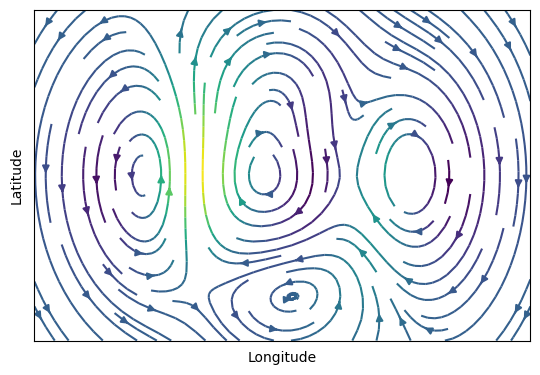
\includegraphics[width=0.7\textwidth]{figure1.png}
    \caption{This is the caption, sandworm vorticity based on storm location in a pleasing stream plot. Based on example in \href{https://matplotlib.org/stable/plot_types/arrays/streamplot.html}{matplotlib}. \label{egfig}}
\end{figure}


\begin{figure}[]
    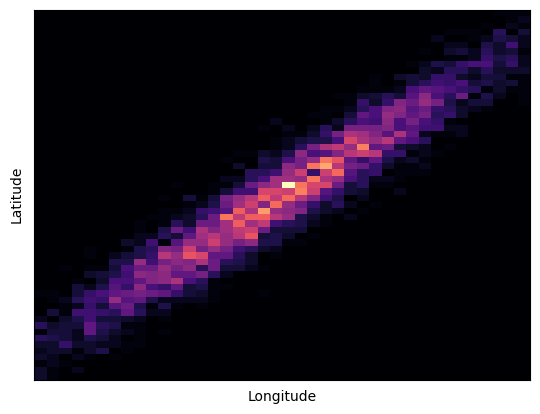
\includegraphics[width=0.7\textwidth]{figure2.png}
    \caption{This is the caption, electromagnetic signature of the sandworm based on remote sensing techniques. Based on example in \href{https://matplotlib.org/stable/plot_types/stats/hist2d.html}{matplotlib}. \label{egfig2}}
\end{figure}

As you can see in \autoref{egfig}, the vorticity is high in the margins. Additionally in Figures \ref{egfig} and \ref{egfig2} ... this is how you reference auto-numbered figures.
Use \texttt{autoref} when referring to a single figure, and \texttt{ref} if you need individual access to the number.

\begin{table}
    \centering
    \caption{This is the caption for the materials table.\label{mtable}}
    \begin{tabular}{cc}
    \toprule
    \textbf{Material} & \textbf{Units} \\
    \midrule
    Stone & 3 \\
    Water & 12 \\
    Cement & $\alpha$ \\
    \bottomrule
    \end{tabular}
\end{table}

We show the different quantities of materials required in \autoref{mtable}.

% The statement below shows how to adjust the width of a table.

\begin{longtable}[c]{p{0.110\textwidth}p{0.02\textwidth}p{0.02\textwidth}p{0.086\textwidth}p{0.086\textwidth}p{0.086\textwidth}p{0.110\textwidth}}
    \caption{This is the caption for the wide table with custom widths.\label{wide-table}} \\
    \toprule
    This & is & a & very & very & wide & table \\
    \bottomrule
\end{longtable}

And since you are working in raw LaTeX already, you can easily make complex
table formats. Above we used \verb|\DUtablewidth| to control the width of individual parts of a table, but you can also let tex worry about that part for you:

\begin{longtable}{|l|rrr|}
\caption{Area Comparisons \label{quanitities-table}}\\
\hline
\multirow{2}{*}{\bf Projection} & \multicolumn{3}{c|}{\bf Area in square miles} \\
\cline{2-4}
& \textbf{Large Horizontal Area} & \textbf{Large Vertical Area} & \textbf{Smaller Square Area} \\
\hline
\endfirsthead
Albers Equal Area & 7,498.7 & 10,847.3 & 35.8 \\
Web Mercator & 13,410.0 & 18,271.4 & 63.0 \\
Difference & 5,911.3 & 7,424.1 & 27.2 \\
Percent Difference & 44\% & 41\% & 43\% \\
\hline
\end{longtable}

Perhaps we want to end off with a quote by Lao Tse\footnote{$\mathrm{e^{-i\pi}}$}:

\begin{quote}
    Muddy water, let stand, becomes clear.
\end{quote}


